\section{Modo Protegido}

\subsection{Selector de Segmento}
Al entrar a modo protegido, inicializamos los diferentes selectores de segmento. Los mismos tienen el siguiente formato:

\begin{figure}[h!]
  \centering
    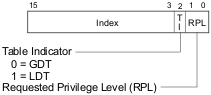
\includegraphics[scale=0.8]{images/segment_selector}
  \caption{Segment Selector}
\end{figure}

El index corresponde a un descriptor de segmento de la \texttt{GDT}. Nosotros no utilizaremos la LDT, por lo que el bit TI estará siempre en 0. Ademas el \texttt{RPL} (Requested Protection Level) estará siempre en nivel 0 (superuser) o en 3 (usuario).

\subsection{Niveles de protección}

Intel soporta 4 niveles de protección diferentes, siendo 0 el mas alto y 4 el mas bajo. Por esa razón los bits de protección tienen 2 bits.

\begin{figure}[h!]
  \centering
    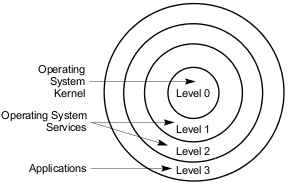
\includegraphics[width=0.3\textwidth]{images/protection_rings}
  \caption{Protection Rings}
\end{figure}

Si el $max(CPL, RPL) > DPL$ (recordemos que un nivel de protección mayor numerico se corresponde a un menor nivel de privilegio) al querer acceder o hacer un salto a un segmento, la \texttt{Unidad de Protección} verifica que no tenemos privilegios suficientes y el procesador nos da un General Protection Fault (\#GP). Esto se puede ver en la siguiente figura:

\begin{figure}[H]
  \centering
    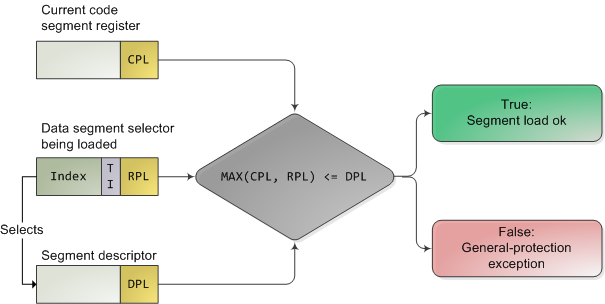
\includegraphics[width=0.6\textwidth]{images/protection}
  \caption{Protection Diagram}
\end{figure}

\subsection{Interrupt Descriptor Table}

Una interrupción es una señal que le indica a la CPU que debe interrumpir la ejecución actual de instrucciones. El rol de la \texttt{IDT} (Interrupt Descriptor Table) es contener los diferentes descriptores de interrupción y asociar las diferentes interrupciones a sus respectivas rutinas de atención de interrupción. Existen tres fuentes de interrupciones:

\begin{enumerate}
\item Hardware
\item Software
\item Internas
\end{enumerate}

A su vez, la \texttt{IDT} puede contener tres tipos de descriptores:

\begin{enumerate}
\item Interrupt Gate
\item Trap Gate
\item Task Gate
\end{enumerate}

Para construir la IDT, armamos primero en C la estructura \texttt{idt\_entry} con sus respectivos atributos y luego construimos un array de 256 posiciones del mismo (la máxima cantidad soportada por el PIC). En este trabajo practico solo utilizaremos descriptores de interrupción y de tarea.

\begin{figure}[h!]
  \centering
    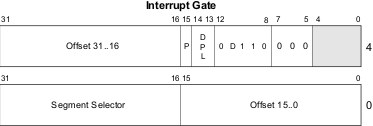
\includegraphics[width=0.5\textwidth]{images/idt_desc}
  \caption{IDT Descriptor}
\end{figure}

Modificamos la macro de la cátedra para poder cargar la IDT con diferentes atributos. Luego inicializamos las diferentes posiciones que utilizamos con sus respectivos selectores de segmento y atributos, tomando también la referencia a las respectivas rutinas de atención.

Hay que tener mucho cuidado al settear los atributos. Caso contrario, al cambiar de segmento podemos tener un General Protection Fault (\#GP). Algunos atributos son:

\begin{enumerate}
\item P: Present flag. 1 if present.
\item DPL: Descriptor Protection Level. Nivel de privilegios del descriptor.
\item D: Size of gate. 1 = 32 bits; 0 = 16 bits.
\end{enumerate}

Un procesador Intel reserva por default las primeras 31 posiciones de la \texttt{IDT} para las diferentes excepciones del procesador. Actualmente, el procesador solo utiliza las primeras 21. Inicializamos estas excepciones del procesador a una rutina que guarda el estado del procesador al suceder la primera interrupción y en caso de ser necesario desaloja la tarea actual. También inicializamos otros descriptores para atender otras interrupciones como la del reloj y la del teclado.

Una vez cargada la IDT, se debe remapear el PIC (Programmable Interrupt Controler) para referir a las nuevas interrupciones que agreguemos. Esto se hace con las rutinas de la cátedra \texttt{resetear\_pic} y luego \texttt{habilitar\_pic}.

\pagebreak

\subsection{Memory Management Unit}
Un procesador Intel, para gestionar lo que son los accesos a memoria, utiliza una \texttt{MMU} (Memory Management Unit). La misma esta compuesta por la Unidad de Segmentación y la Unidad de Paginación. La siguiente figura ilustra la idea general:

\begin{figure}[H]
  \centering
    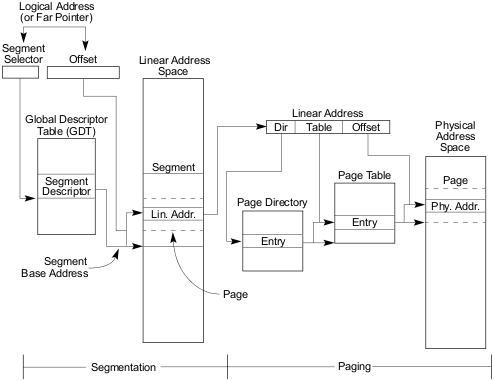
\includegraphics[width=0.4\textwidth]{images/memory_management}
  \caption{Segmentation \& Paging}
\end{figure}

La paginación nos permite que cada tarea pueda tener su propia \texttt{memoria virtual}, mappeando direcciones virtuales a direcciones físicas.

\subsubsection{Unidad de Segmentación}

La unidad de segmentación se ocupa de pasar desde las \textit{direcciones lógicas} a direcciones lineales. Para ello, utiliza la GDT para identificar el segmento adecuado y luego su respectivo offset. La unidad de protección verifica que el \texttt{DPL} es compatible con el \texttt{CPL} y el \texttt{RPL}.

En modo protegido, los selectores de segmento tienen 16 bits. Los 13 bits mas significativos contienen el indice dentro de la tabla de descriptores. El bit 2 especifica si la operación utiliza la \texttt{GDT} o la \texttt{LDT}. Finalmente, los 2 bits menos significativos definen el nivel de privilegio solicitado.

\subsubsection{Unidad de Paginación}

Para activar la paginación, en primer lugar debemos inicializar el directorio de paginas y cargar el registro \reg{cr3} con la dirección del mismo. Como los directorios de paginas están alineados a 4 kb, los primeros 12 bits del \reg{cr3} no son necesarios para identificar el directorio, por lo que son utilizados por atributos del procesador. En nuestro caso no utilizamos estos atributos, por lo que son todos 0. La siguiente tabla muestra el formato del \reg{cr3}.

\begin{figure}[H]
  \centering
    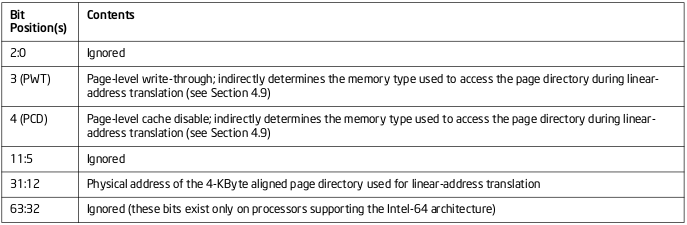
\includegraphics[width=0.8\textwidth]{images/cr3}
  \caption{CR3 Format}
\end{figure}

Luego activamos la paginación con el ultimo bit del registro \reg{cr0}. Una vez activada, la dirección lineal comienza a pasar luego por la unidad de paginación. La unidad de paginación se encarga de ir desde la dirección lineal a la dirección física en memoria. En caso de que la dirección lineal no este paginada, el procesador tiene una Page Fault Exception (\#PF).

\subsection{Otras Interrupciones}

Para inicializar otras interrupciones, tenemos que agregar los diferentes descriptores a la IDT, que apuntan a su correspondiente rutina de atención y ademas tienen los atributos correctos. Recordemos que las rutinas de atención de la interrupción deben ser transparentes a lo que el procesador estaba ejecutando en el momento, por lo que se deben guardar todos los registros utilizados y luego restaurarlos al finalizar la rutina de atención. Ademas, las interrupciones en general llevan a un escalamiento de privilegios, por lo que los privilegios también deben ser restaurados.

A su vez, la rutina de atención de la interrupción debe indicarle al pic que la interrupción esta siendo atendida, para que otras interrupciones puedan suceder. Esto se hace con la rutina de la cátedra \fun{fin\_intr\_pic1}.

\subsubsection{Reloj}

Esta es una interrupción interna, que sucede con cada \texttt{tick} del reloj del procesador. La rutina de atención de esta interrupción se encarga de mostrar la animación de un cursor rotando en la esquina inferior derecha de la pantalla, por medio de la función \fun{screen\_actualizar\_reloj\_global}. Luego haremos que llame al Scheduler y haga el switch de tareas.

\subsubsection{Teclado}
Utilizaremos la rutina de atención del teclado para habilitar las diferentes teclas disponibles a los jugadores. Cuando programábamos esto, notamos que es necesario tomar la tecla presionada desde el controlador del teclado, caso contrario el teclado no vuelve a solicitar una interrupción.

\subsubsection{Software}
Asignamos a la interrupción \addr{0x46} (70) una rutina que atiende un servicio del sistema.

\subsection{Task State Segment}

La \texttt{TSS} (Task State Segment) es el espacio de memoria previsto en los procesadores \texttt{IA-32} como el espacio de contexto de cada tarea. Este segmento debe tener su respectivo descriptor en la \texttt{GDT}. 

\begin{figure}[H]
  \centering
    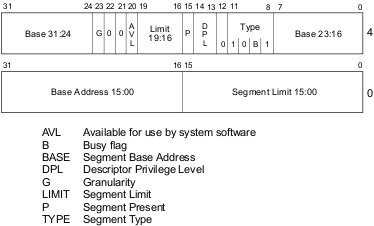
\includegraphics[width=0.5\textwidth]{images/tss_descriptor}
  \caption{TSS Descriptor}
\end{figure}

Este descriptor apunta a un segmento con la siguiente estructura:

\begin{figure}[H]
  \centering
    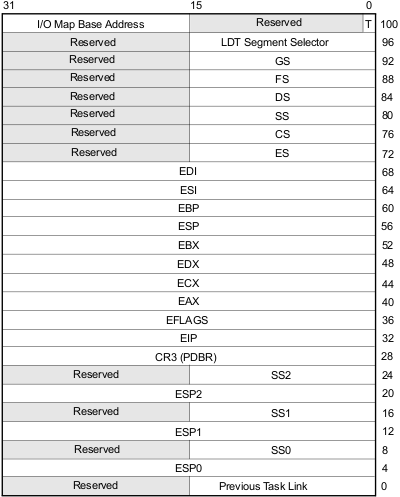
\includegraphics[width=0.3\textwidth]{images/tss}
  \caption{Task State Segment}
\end{figure}

Estas estructuras deben ser inicializadas con cuidado, con sus respectivos \reg{EIP}, \reg{ESP}, \reg{EBP}, \reg{CR3} e \reg{EFLAGS} entre otros. Por ejemplo, para que las interrupciones esten habilitadas \reg{EFLAGS} debe tener el valor \hex{0x202}.

Ademas, el selector de segmento de la tarea que se
esta ejecutando actualmente se debe encontrar en el registro \reg{TR} (Task Register). Este selector tiene 16 bits. Ademas, este registro tiene una parte oculta que cachea el descriptor de segmento correspondiente al selector. Las instrucciones \texttt{LTR} y \texttt{STR} nos permiten cargar y guardar el Task Register solo si tenemos \texttt{CPL} 0.

\begin{figure}[H]
  \centering
    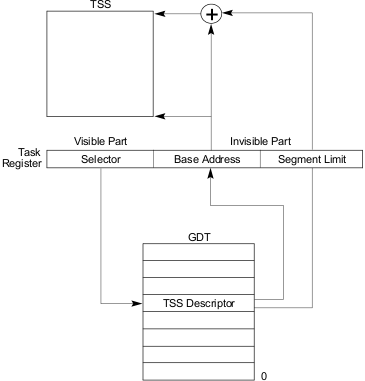
\includegraphics[width=0.3\textwidth]{images/task_register}
  \caption{Segmentation \& Paging}
\end{figure}

Para llamar a una tarea, se lleva a cabo un \texttt{jump far} con su respectivo selector de segmento (el offset no se utiliza). El procesador guarda el contexto de la tarea actual en la TSS correspondiente al \reg{TR}, y se carga el nuevo contexto de ejecución. 

La primera vez que llamamos a una tarea, el registro \reg{TR} no tiene un valor definido. Por esta razon definimos la \texttt{tss\_inicial} y cambiamos el \reg{TR} antes de saltar a la primera tarea.